\begin{figure}[h!]
\centering
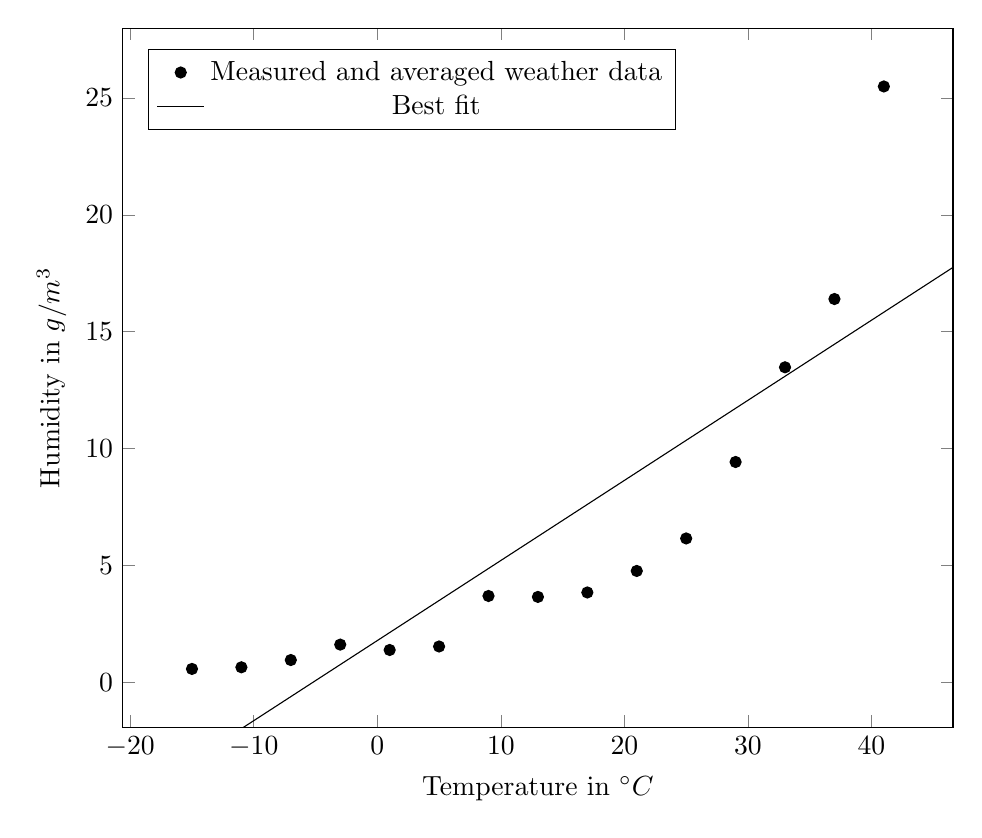
\begin{tikzpicture}
\begin{axis}
[ xlabel = Temperature in $ ^{\circ} C$,
ylabel = Humidity in $g/m^3$,
legend pos = north west,
xmin=-20.6, xmax=46.6,
ymin=-1.911, ymax=27.980999,
width=1\textwidth
]
\addplot[
only marks,
error bars/.cd,
 y dir=both,y explicit,
x dir=both,x explicit,
]
coordinates{
(-15,0.58) +- (0,0)
(-11,0.65) +- (0,0)
(-7,0.96) +- (0,0)
(-3,1.62) +- (0,0)
(1,1.39) +- (0,0)
(5,1.54) +- (0,0)
(9,3.7) +- (0,0)
(13,3.66) +- (0,0)
(17,3.85) +- (0,0)
(21,4.77) +- (0,0)
(25,6.16) +- (0,0)
(29,9.43) +- (0,0)
(33,13.48) +- (0,0)
(37,16.4) +- (0,0)
(41,25.49) +- (0,0)
};
\addlegendentry{Measured and averaged weather data}
\addplot[
domain=-20.6:46.6,
]
{x*0.34252678571428574 + 1.792485119047619}
;
\addlegendentry{Best fit}
\end{axis}
\end{tikzpicture}
\caption{Environment data of one year by a franconian weather station Thomas Karb 11.5.23}
\label{fig:EnvironmentRegression}
\end{figure}
